%!TEX root = ../VorlageBA.tex
\chapter{Kapitel Zwei}
Hier würde eine Einleitung zum Kapitel stehen... 

\section{Abbildungen in LaTeX}
\label{sec:abbildungen_in_latex}

Beispiel für eine Grafik:
\begin{figure}[!ht]
	\centering
		%[natürliche Breite in Pixeln, natürliche Höhe in Pixeln, Abhängigkeit von der Textbreite]
		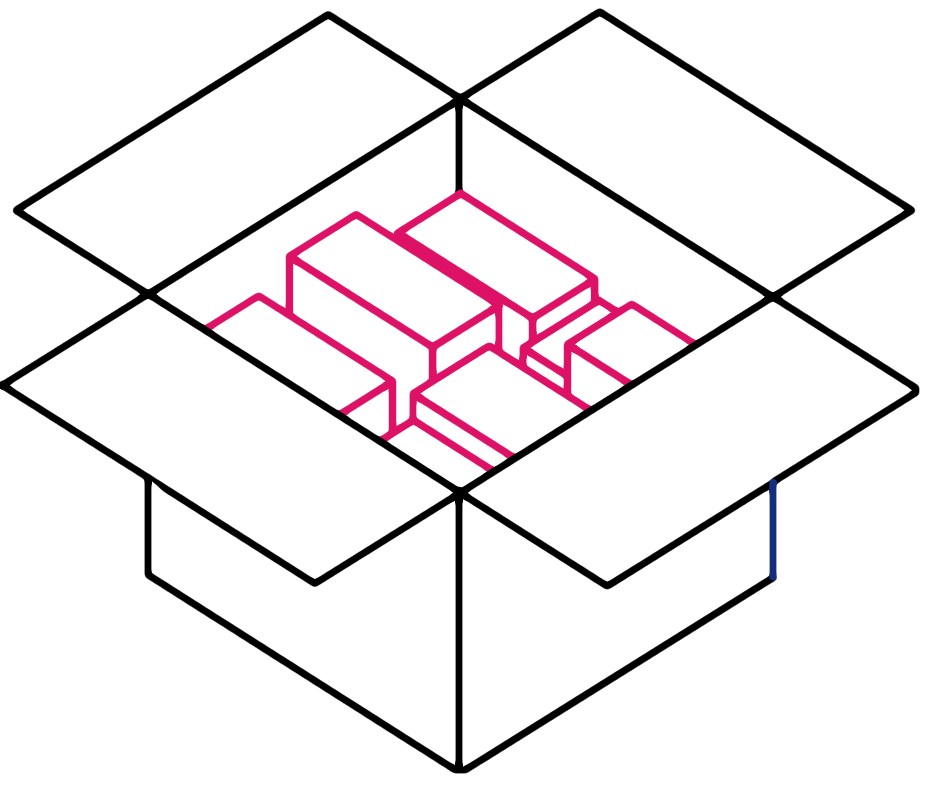
\includegraphics[width=0.75\textwidth]{images/MIBox.png}
	\caption{Bildunterschrift mit einer Quelle \citep{Autor2013}}
	\label{fig:box}
\end{figure}

Eine Abbildung sollte immer im Text diskutiert werden und dann entsprechend mit dem \texttt{ref{}}-Befehl referenziert werden. Bitte beachten Sie auch, dass die Quelle entsprechend angegeben wird. An dieser Stelle wurde exemplarisch mit dem \texttt{cite{}} Befehl ein Quelle hinzugefügt.

\section{Zitierweise}
Dies ist ein Beispiel für ein wörtliches Zitat:
\begin{quotation}
	\emph{``A persona is a rich picture of an imaginary person who represents your core user group.''} \citep{Dix04}
\end{quotation}

Alternativ könnte man auch schreiben: 
\begin{quotation}
	\textit{\enquote{A persona is a rich picture of an imaginary person who represents your core user group.}} \citep{Dix04}
\end{quotation}

Das Ergebnis im Dokument ist hier gleich. \\

Manchmal möchte man die Autorennamen im Text verwenden. Bislang haben wir den \texttt{citep\{\}} Befehl verwendet. Hierdurch werden die Klammern um Autorname und Jahr gesetzt. Man kann den \texttt{cite} Befehl allerdings auch variieren: \\

\cite{Dix04} definieren das Konzept "Persona" wie folgt: 
\begin{quotation}
	\emph{``A persona is a rich picture of an imaginary person who represents your core user group.''}
	\citep{Dix04}
\end{quotation}

Das richtige Setzen der Klammern erhöht die Lesbarkeit. \\

Im APA Format\footnote{ American Psychological Association (APA)} gibt es einige Regeln, wann und wie man Seitenzahlen bei den Literaturverweisen verwendet:

\begin{quotation}
	\emph{``Include page numbers for any citations in the text of your paper that include direct quotations or refer to a specific part of the work you are referencing. Direct quotations must include a page number as part of the citation. The quoted material should be followed by a citation in parentheses that gives the author's name, the year in which the work was published, and the page number from which the quoted material appears.''}
	\citep{Hall}
\end{quotation}

Weitere Beispiele und Empfehlungen von \cite{Hall} finden Sie hier:  \url{http://www.ehow.com/how_5689799_cite-numbers-apa-format.html}. In \LaTeX{} kann man die Seitenzahlen sehr einfach hinzufügen, zum Beispiel: \\

\citet[S. 86]{Baddeley:1974ts} führen aus: 

\begin{quotation}
	\emph{``We hope that our preliminary attempts to begin answering the question will convince the reader, not necessarily that our views are correct, but that the question was and is well worth asking''}
	\citep[p. 86]{Baddeley:1974ts}
\end{quotation}

Im ersten Verweis auf \citeauthor{Baddeley:1974ts} haben wir \texttt{citet[]\{\}} verwendet, um die Klammern um das Jahr zu setzen. Im zweiten Fall im Anschluss an das Zitat wurde \texttt{citep[]\{\}} verwendet.

\section{Verweise innerhalb des Dokumentes} % (fold)
\label{sec:verweise_im_dokument}

Wenn Sie auf Ihre eigenen Kapitel, Abbildungen, Tabellen o.ä. verweisen wollen, können Sie den \texttt{ref\{\}} Befehl verwenden, wie auch bereits vorab gezeigt im Abschnitt~\ref{sec:tabellen_ref} auf Seite~\pageref{sec:tabellen_ref}.  \\

An dieser Stelle möchten wir nun auf die MI Box verweisen. Sie hat die Abbildungsnummer~\ref{fig:box} und ist auf Seite \pageref{fig:box} zu finden. Wie Sie an diesem Beispiel auf dieser Seite sehen, kann man mit \LaTeX{} nicht nur auf die Abschnitts-/ oder Tabellennummer verweisen, sondern auch auf die Seitenzahl auf der das Label verweist. Wenn Sie diese dynamischen Codes verwenden (statt zum Beispiel die Nummerierung manuell einzutragen), haben Sie immer die korrekte Nummerierung, auch wenn Sie den Text später umstrukturieren. Wir nutzen den \texttt{pageref\{\}} Befehl hierfür.

% section verweise_im_dokument (end)



